% Chapter 1

\chapter{Introducción general} % Main chapter title

\label{Chapter1} % For referencing the chapter elsewhere, use \ref{Chapter1} 
\label{IntroGeneral}

%----------------------------------------------------------------------------------------

% Define some commands to keep the formatting separated from the content 
\newcommand{\keyword}[1]{\textbf{#1}}
\newcommand{\tabhead}[1]{\textbf{#1}}
\newcommand{\code}[1]{\texttt{#1}}
\newcommand{\file}[1]{\texttt{\bfseries#1}}
\newcommand{\option}[1]{\texttt{\itshape#1}}
\newcommand{\grados}{$^{\circ}$}

%----------------------------------------------------------------------------------------

%\section{Introducción}

%----------------------------------------------------------------------------------------
En este capítulo se realiza una introducción a la realidad aumentada y los sistemas de control distribuidos. Además, se explica la motivación, alcance y objetivos del presente trabajo.

\section{Realidad aumentada}

Las tecnologías que permiten que un usuario visualice parte del mundo real a través de un dispositivo tecnológico se pueden clasificar en realidad virtual, realidad aumentada y realidad mixta. En la figura \ref{fig:realidades} se ilustran cada una de estas tecnologías.

\begin{figure}[htpb]
	\centering
	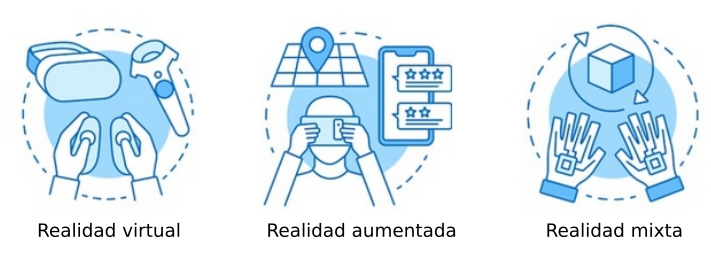
\includegraphics[width=\textwidth]{./Figures/realidades.png}
	\caption{Clasificación de tecnologías\protect\footnotemark.}
	\label{fig:realidades}
\end{figure}

\footnotetext{Imagen tomada de \url{https://scand.com/company/blog/augmented-mixed-and-virtual-reality-for-business/}}

La realidad virtual, consiste en un ambiente completamente digital. Se buscan aislar los sentidos del usuario del mundo real. De esta manera el usuario queda inmerso en otra realidad con la cual puede interactuar. Los dispositivos que permiten esta interacción son los cascos de realidad virtual y sus \textit{joysticks}.

La realidad aumentada es una tecnología que permite conectar los dos mundos, el mundo físico y el mundo digital. Esto se logra superponiendo imágenes sobre la percepción que el usuario tiene del mundo real, mediante el uso de hologramas o incluso con teléfonos celulares. De esta forma en la pantalla se muestra no sólo el ambiente en el que esta el usuario, sino que además se proyecta información adicional. Ejemplos de esta tecnología son los populares filtros de Instagram o el juego PokemonGo.

Por último, la realidad mixta es una mejora de la realidad aumentada. Los elementos no sólo son adicionados sobre la percepción visual, sino que interactúan además con el espacio físico. Por ejemplo, si tuviéramos una pelota en una aplicación de realidad mixta, la misma podría rodar cuesta abajo de una escalera.

\section{Aplicaciones de realidad aumentada en la industria}

A continuación se presenta un listado de algunos trabajos contemporáneos relacionados con la realidad aumentada y su aplicación en la industria.

\subsubsection{\textit{Smart retrofitting in the context of industry 4.0}}
En este trabajo publicado en Elsevier \citep{MX1}, se utiliza el Hololens 2 para capacitar a los operadores luego de una mejora en una máquina dobladora de caños. El trabajo destaca que la herramienta permite a los operadores adaptarse rápidamente a la máquina, permitiéndoles trabajar de manera segura y guiada.

\subsubsection{\textit{Production workplace enhanced by mixed reality}}
En este paper presentado en la conferencia \textit{Mensch und Computer} 2020 en Alemania \citep{MX2}, se muestra una aplicación de realidad aumentada para guiar al operador en el ensamblado de un scooter. El trabajo destaca el análisis de la relación costo-beneficio a la hora de armar procedimientos para los operadores. Plantean que deben encararse soluciones de realidad aumentada, donde el beneficio sea considerable, dado que estas aplicaciones requieren un elevado tiempo de desarrollo.

\subsubsection{\textit{Mixed reality technology for onsite construction assembly}}
En este paper presentado en la conferencia \textit{Materials Science, Engineering and Chemistry} 2020 \citep{MX3}, se presenta una aplicación de realidad aumentada cuyo objetivo es comunicar los detalles de diseño para el montaje y la construcción. El trabajo destaca que el Hololens 2 es capaz de guiar la instalación de componentes eléctricos y de plomería, logrando un 9\% de mejora en la productividad. Menciona además, que las imágenes ocluidas en condiciones de luz solar, son el desafío a superar por el HoloLens 2 antes de una adopción generalizada.

\section{Procedimientos \textit{batch}}

Un procedimiento \textit{batch} o por lotes es aquel donde el producto sufre modificaciones consecutivas con el correr del tiempo\citep{Batch:1}. El producto avanza por distintas etapas hasta estar terminado. En ese momento se evacua el producto de la instalación, se carga producto base y el ciclo comienza nuevamente. En la figura \ref{fig:tanks} se puede ver que en el proceso por lotes, sólo cuando se llega a t=4 se obtiene el producto final deseado. Mientras que en el proceso continuo, el tanque contiene producto terminado desde el momento inicial t=0.

\begin{figure}[htpb]
	\centering
	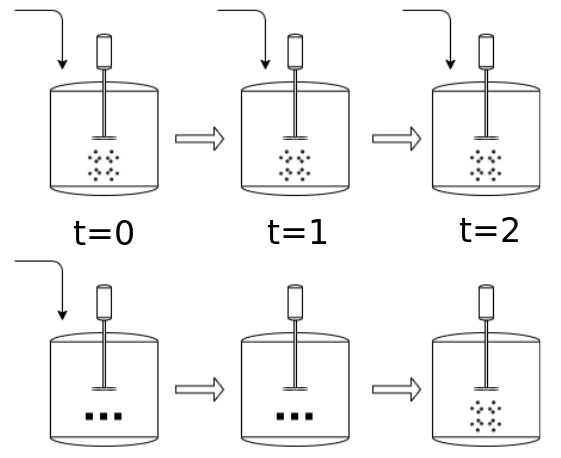
\includegraphics[scale=.45]{./Figures/tanks.png}
	\caption{Proceso continuo (superior) vs proceso por lotes (inferior).}
	\label{fig:tanks}
\end{figure}

Algunas operaciones por lotes implican el uso de hojas de cálculo. Por ejemplo, un operador puede agregar una bolsa de químicos a un reactor y luego agregar un segundo químico. La razón entre el segundo y el primero debe ser exacta. Se necesita entonces una hoja de cálculo para determinar la cantidad requerida del segundo producto. 

Los procedimientos operativos para los procesos por lotes son generalmente más complicados y difíciles de escribir que para las instalaciones de proceso continuo porque el tiempo es un factor. Además, muchas instalaciones están diseñadas para fabricar varios productos partiendo de los mismas maquinas en producción. Por lo tanto, se necesitan dos o más procedimientos para los mismos equipos de la planta, lo que da lugar a confusiones y malentendidos en los operadores.

\section{DCS utilizado en el trabajo}

Los sistemas de control distribuidos, también conocidos por sus siglas en inglés DCS \citep{DCS}, son sistemas compuestos por sensores, controladores y computadoras que se distribuyen por toda la planta. Cada uno de estos elementos tiene un propósito único, como la adquisición de datos, el control de procesos, el almacenamiento de datos o la visualización gráfica. Estos elementos individuales se comunican con un sistema centralizado a través de la red de área local de la planta, denominada red de control. En la figura \ref{fig:800xA}, la arquitectura de red del sistema DCS de ABB \citep{DCSaq}, usado en este trabajo.

\begin{figure}[htpb]
	\centering
	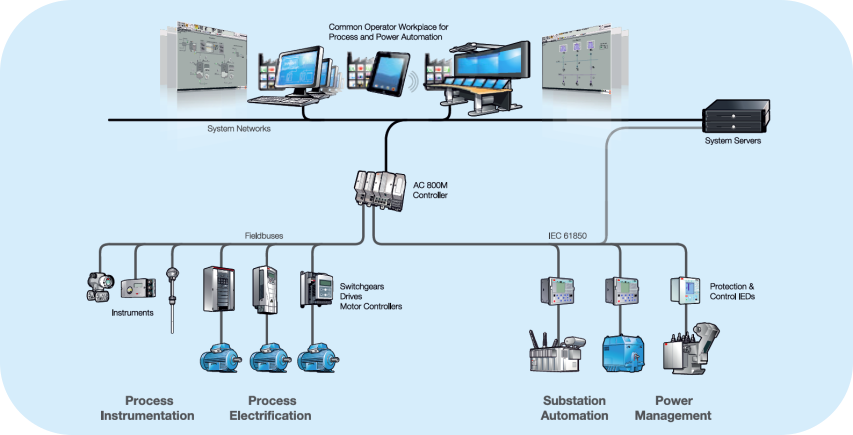
\includegraphics[scale=.45]{./Figures/800xA.png}
	\caption{Sistema de control distribuido 800xA\protect\footnotemark.}
	\label{fig:800xA}
\end{figure}

\footnotetext{Imagen tomada de \url{https://new.abb.com/control-systems/system-800xa/800xa-dcs/system/architecture}}
\vspace{70px}

El DCS toma decisiones automatizadas basadas en las tendencias de producción de toda la planta. Como ejemplo, el DCS de una planta de energía, podría aumentar automáticamente la capacidad de generación de vapor de múltiples turbinas, para adecuarse a la demanda cambiante de electricidad. Mientras que un PLC puede ajustar la operación de una sola unidad, el DCS puede realizar ajustes en cada una de las unidades de control que interactúan en una planta.\\

Como sistema de control en este trabajo, se utilizó la herramienta de ABB denominada \textit{SoftController} \citep{softc}. Esta nos permite simular la presencia de un controlador físico conectado a la red, con la IP del localhost. El CBM (\textit{Compact Control Builder}) \citep{cbm}, permite crear lógicas del mismo tipo que las usadas en los sistemas DCS 800xA de ABB. De hecho las mismas podrían exportarse al sistema 800xA sin problemas. A continuación se puede ver la figura \ref{fig:c1} del \textit{SoftController} simulando un controlador.

\begin{figure}[htpb]
	\centering
	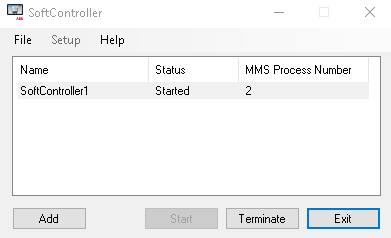
\includegraphics[scale=.6]{./Figures/c1.png}
	\caption{Controlador simulado\protect\footnotemark.}
	\label{fig:c1}
\end{figure}

Por último tenemos el OPC server. Ésta aplicación crea un OPC server para acceder a las variables del sistema de control. Para conectarnos debemos apuntar a la IP del controlador simulado como se muestra en la figura \ref{fig:c2}.

\begin{figure}[htpb]
	\centering
	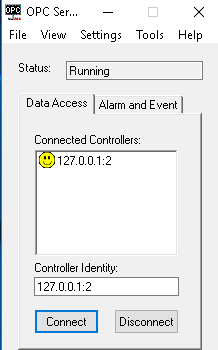
\includegraphics[scale=.5]{./Figures/c2.png}
	\caption{OPC server\protect\footnotemark.}
	\label{fig:c2}
\end{figure}

%----------------------------------------------------------------------------------------

\section{Motivación}
El propósito de este trabajo es innovar en la interacción entre los operadores y los sistema de control distribuidos, para impulsar nuevas soluciones en el área de la automatización industrial. Se busca explorar las oportunidades que ofrece la realidad aumentada para mejorar y optimizar las tareas de los operadores, además de agilizar el entrenamiento de nuevos operarios y mejorar la seguridad para procedimientos bajo situaciones de emergencia.

%----------------------------------------------------------------------------------------

\section{Alcance}

En la presente memoria, se documenta el trabajo realizado donde se incluyen los siguientes aspectos:

\begin{itemize}	
\item Desarrollo de la aplicación de realidad aumentada.
\item Desarrollo del conector OPC.
\item Desarrollo de API REST.
\item Comunicación entre el DCS y la interfaz holográfica.
\item Implementación de base de datos cloud.
\end{itemize}